%% CAPITULO 2
\hypertarget{estilo:capitulo}{}
\chapter{REVISÃO BIBLIOGRÁFICA}

\section{Assimilação de Dados}
\label{ss:assimdados}

O processo de previsão numérica do tempo pode ser entendido como um problema de valor inicial e de contorno, no qual as equações governantes são integradas no tempo (e. g., equações 1.1, 1.2 e 1.3). As condições iniciais determinam como o modelo de previsão iniciará o ciclo de análise (equação 2.1). As condições de contorno determinam como serão os ciclos de previsão (equação 2.2), sendo portanto, muito importantes durante todo o tempo de integração do modelo (NOWOSAD, 2001). Para tanto, utilizam-se como condição inicial valores bem determinados dos campos meteorológicos em um dado instante de tempo e como condição de contorno, valores compatíveis em física e dinâmica com o modelo de previsão. Segundo TALAGRAND (1997), a AD pode ser definida como a forma mais acurada possível de se reconstruir o fluxo atmosférico utilizando todas as informações disponíveis no momento de sua geração.

\begin{equation}
\textit{\textbf{w}}^{f}_{n}=\textit{\textbf{F}}[\textit{\textbf{w}}^{a}_{n-1}]
 \label{form04}
\end{equation}

\begin{equation}
\textit{\textbf{w}}^{f}_{a}=\textit{\textbf{w}}^{f}_{n}+\textit{\textbf{d}}_{n}
 \label{form05}
\end{equation}

Onde:

\begin{itemize}
\item $\textit{\textbf{w}}_{n}$: representa o vetor de variáveis de estado no passo temporal \textit{n};
\item $\textit{\textbf{F}}[.]$: representa o modelo de PNT;
\item $\textit{\textbf{d}}_{n}$: é o vetor de inovação da análise, o qual contém informações derivadas das observações.
\end{itemize}

Os índices $\textit{f}$ e $\textit{a}$ denotam os valores previstos e analisados, respectivamente.

A condição inicial utilizada nos modelos de PNT é constituída por um conjunto de observações, convencionais (de superfície e ar superior) e não convencionais (de satélites), as quais são providas nos quatro horários sinóticos padrões (00Z, 06Z, 12Z e 18Z) e por um campo de first guess, uma previsão de curto prazo de tipicamente 6 horas. Todas estas informações são combinadas de forma ótima e constituem a análise que é a condição inicial dos modelos de PNT. Operacionalmente, como por exemplo, no CPTEC, essas observações são utilizadas nos horários das 00Z e 12Z (Figura 1.3). Estes são os horários em que as observações são mais abundantes sobre a América do Sul e em que são feitas as previsões operacionais do centro.

Segundo MOREL 1980, em uma situação física ideal, pode-se esperar que as observações (que são informações sinóticas) determinem um valor para cada parâmetro meteorológico (e.g. temperatura, pressão à superfície e ventos). No entanto, observa-se que isto não acontece devido a vários fatores:

\begin{itemize}
\item As observações de temperatura, pressão à superfície e ventos são distribuídas de forma muito irregular na terra e deixam muitas dúvidas sobre regiões onde não há observações;
\item As observações convencionais são medidas pontuais que não são representativas dos campos meteorológicos de volumes médios, tais como os modelos de PNT requerem.
\end{itemize}

Além disso, observações convencionais estão sujeitas a erros grosseiros dos instrumentos. Por outro lado, temos as observações não convencionais (que são informações assinóticas ou remotas), as quais podem fornecer mais detalhes sobre o fluxo atmosférico. No entanto, estes tipos de observações também possuem as suas limitações:

\begin{itemize}
\item As observações não convencionais, a partir do espaço, determinam de forma indireta perfis verticais de temperatura e podem proporcionar uma cobertura homogênea contínua de 6 a 12 horas. Estes tipos de observações são não sinóticas, mas são distribuídas no espaço e no tempo. Porém são os satélites, síncronos com o Sol, que as provém. O aproveitamento destas informações em modelos numéricos de PNT torna-se, portanto, incompleta;
\item As observações remotas dos movimentos das nuvens a partir de satélites geoestacionários são capazes de disponibilizar dados em horários sinóticos e prover uma amostragem horizontal dos campos de vento. Porém, a resolução vertical destes tipos de observações se limita a um ou dois níveis verticais, o que pode ser insuficiente para os modelos.
\end{itemize}

Estes tipos de observações, sempre incluem considerações físicas e algoritmos sofisticados de processamento de dados para reconstruir os parâmetros meteorológicos, a partir de quantidades medidas remotamente. Estes procedimentos têm a sua própria deficiência e podem causar erros aleatórios e/ou sistemáticos.

Desta forma, pode-se concluir que o conjunto de dados que se tem disponível para uso com os modelos de PNT, pode ser incompleto e insuficiente para uma descrição adequada do fluxo atmosférico global. Por outro lado, o uso combinado de observações convencionais (sinóticas) e não convencionais (assinóticas), mostra-se mais interessante por formar um conjunto de dados mais consistente para uso como condição inicial nos modelos de PNT. No CPTEC, operacionalmente utilizam-se observações sinóticas e assinóticas para a inicialização do modelo regional Eta, as quais são interpoladas na grade do modelo utilizando-se um sistema de análise estatística em espaço físico (espaço das observações - PSAS).

Qualquer modelo de PNT precisa ser inicializado (ou iniciado) mesclando-se as observações com os campos estimados atuais, calculados com base em observações de um instante de tempo passado. Formalmente, este problema consiste em otimizar a integração do modelo (considerando-o como um sistema com  graus de liberdade, ou seja, com  variáveis), enquanto adicionam-se todas as informações atuais disponíveis. Esse processo de mesclar-se as novas observações com o resultado da integração do modelo de PNT é conhecido como Assimilação de Dados Quadrimensional ou 4DDA - Four Dimensional Dada Assimilation, em consideração à base espaço-temporal dos dados (latitude, longitude, níveis verticais de pressão e o tempo).

Historicamente, o desenvolvimento das metodologias de AD passou por três estágios principais (WANG et al., 2000, e KALNAY 2003) :

\begin{itemize}
\item Análise Simples: um estágio muito inicial durante década de 1950, enquanto não havia computadores suficientemente rápidos. Os métodos de Análise Simples foram as bases da AD moderna. Nesta década a Análise Simples envolvia técnicas simples de interpolação de dados como Correções Sucessivas, Relaxação Newtoniana e Nudging;
\item Estatística e Interpolação Ótima: considerações estatísticas (baseadas na Teoria da Estimação) foram introduzidas na análise atmosférica e na AD, durante as décadas de 1960 e 1970. Baseadas nestas considerações, métodos baseados em IO foram utilizados para assimilar dados observados em modelos de PNT. Tais métodos de IO foram muito utilizados em vários centros operacionais ao redor do mundo;
\item Análise Variacional: nas décadas de 1980 e 1990 os métodos de assimilação foram substituídos por métodos variacionais como os sistemas de análise multivariacionais (3DVAR, em três dimensões e o 4DVAR em quatro dimensões) utilizando modelos adjuntos. 
\end{itemize}

Em geral, o approach destas técnicas é combinar, de forma ótima, as informações de observações e first guess para produzir a melhor estimativa possível da condição inicial do modelo.

Todos esses esquemas de assimilação evoluíram de acordo com o poderio computacional desenvolvido e adquirido ao longo do tempo. Embora a teoria estatística, que serve de base para praticamente todos os esquemas de AD, já existisse desde os seus primórdios, foi o desenvolvimento de computadores e arquiteturas mais velozes, robustas e flexíveis que permitiram a paralelização e otimização dos esquemas. Este desenvolvimento também possibilitou que a AD fosse desenvolvida no ramo da previsão por ensemble (por conjunto) e também na geração dos algoritmos utilizados por este tipo de esquema.

\section{Ciclo de Assimilação de Dados}
\label{ss:cicloassimdados}

O Ciclo de Assimilação de Dados (CAD) pode ser definido como um sistema retro-alimentador que obtém uma nova análise a partir de informações previamente inseridas no modelo. Há vários métodos de AD e, portanto, diferentes esquemas utilizados em diversos centros operacionais de PNT.

De forma geral, o CAD, pode ser dividido em 4 partes essenciais a todos os diferentes esquemas de assimilação (NOWOSAD, 2001):

\begin{itemize}
\item Controle de Qualidade: no início do CAD, são verificados os dados observados em termos de consistência espaço-temporal. Os dados são comparados com os seus vizinhos e são verificados erros de codificação e de localização dos sensores. Nesta etapa os dados podem ser rejeitados ou não;
\item Análise Objetiva: nesta parte os dados observados são interpolados na grade do modelo e são feitas pequenas correções nos campos previstos do first guess
\item Inicialização: nesta etapa, a partir da análise, são calculadas as condições iniciais de integração as quais são livres de oscilações ou ondas espúrias (e.g. ondas de gravidade inercial). Este processo consiste da utilização de um filtro, responsável pelo processo de inicialização  dos dados inseridos no modelo;
\item Previsão de Curto Prazo: nesta parte é gerado o first guess. Nesta etapa utiliza-se um sistema de assimilação para preparar o próximo estado do modelo. Este sistema inclui as parametrizações necessárias para assegurar que, se não for atualizado com novas observações, o estado por ele gerado será próximo do verdadeiro. Isto garante que na falta de dados, o first guess produzido pelo sistema de AD permaneça plausível.
\end{itemize}

A Figura 2.1 representa o esquema de um CAD intermitente, onde podem ser observadas as diferentes partes do esquema:

\begin{figure}
\centering
\includegraphics[height=7cm]{./figs/fig04.png}
\caption{Ciclo de Assimilação de Dados. Fonte: figura à esquerda, De MATTOS 2006. No processo de assimilação de dados, as informações são extraídas das observações - comumente esparsas, para reconstruir e/ou ajustar a estrutura das variáveis que representam os sistemas atmosféricos. A técnica combina o estado da atmosfera anteriormente predita por uma previsão de curto prazo (first guess), normalmente de 6 horas - (1A na figura à esquerda), com dados observacionais recentes (1B na figura), para produzir um estado atmosférico estimado e atualizado (análise - 4 na figura) e que é usado como condição inicial a partir da qual se gera uma nova previsão.}
\FONTE{KALNAY 2003.}
\label{fig04}
\end{figure}

\section{Sistema Regional de Análise Estatística em Espaço Físico}
\label{ss:rpsas}

No CPTEC, o atual sistema operacional de AD é o Physical-space Statistical Analysis System (PSAS) T213L42 - com 213 ondas no Equador (~ 60 km de resolução horizontal) e 42 níveis verticais, sendo sigma a coordenada vertical. No contexto regional, é utilizado o Regional Physical-space Statistical Analysis System (RPSAS) que é derivado do sistema PSAS desenvolvido pela divisão de assimilação de dados da National Aeronautics and Space Administration (NASA) (Da SILVA et al. 1995; COURTIER 1997). Operacionalmente, o RPSAS é utilizado pelo CPTEC com 40 km de resolução espacial, para produzir a análise utilizada pelos modelos regionais do centro (Eta e BRAMS).

O sistema de assimilação de dados RPSAS é a versão regional desenvolvida e mantida pelo CPTEC em parceria com o Global Modeling and Assimilation Office (GMAO) da NASA. O RPSAS utiliza o mesmo sistema de geração da análise do Global Physical-space Statistical Analysis System (GPSAS) (Da SILVA et al., 1995; COHN et al., 1998). O RPSAS é considerado um esquema com características de 3DVAR e de IO, porém sem as limitações globais do algoritmo do 3DVAR. Estas características permitem que o sistema realize boa parte dos seus cálculos no local onde as observações se encontram e não globalmente, tornando o sistema computacionalmente mais econômico. 

O RPSAS é executado de forma experimental com 20 km de resolução espacial em conjunto com o modelo regional Eta principalmente para previsões de tempo de curto prazo. O sistema é capaz de utilizar dados convencionais provenientes do Global Telecommunication System (GTS), tais como SYNOP, TEMP, SATOB entre outros, além de dados de satélite (QuikSCAT, TRMM, ATOVS e AIRS).

\section{Equação de Inovação e de Análise}
\label{ss:eqinovanl}

O RPSAS utiliza como núcleo de análise o próprio PSAS, sendo que as equações de análise e inovação são resolvidas para o caso regional. Para calcular as inovações trazidas pelas observações e como forma de calcular a análise, são utilizadas as seguintes equações (adaptado de LARSON et al., 1999):

\begin{equation}
(HP^{f}H^{T}+R)X=\textit{\textbf{w}}^o-H\textit{\textbf{w}}^f
\label{form06}
\end{equation}

\begin{equation}
\textit{\textbf{w}}^a-\textit{\textbf{w}}^f=P^{f}H^{T}X
\label{form07}
\end{equation}

Onde:

\begin{equation}
X^{a}=X^{b}+W[y^{o}-H(X^{b})]
\label{form08}
\end{equation}

Onde:

\begin{itemize}
\item $P^{f}$: é a matriz (de ordem $n$) de covariância dos erros da previsão;
\item $R$: é a matriz (de ordem $p$) de covariância dos erros de observação;
\item $H$: é uma matriz de ordem $p$$\times$$n$ que interpola as observações na grade no vetor previsão (em ponto de grade);
\item $\textit{\textbf{w}}^o$: é o vetor das observações, de ordem $p$;
\item $\textit{\textbf{w}}^f$: é o vetor previsão (em ponto de grade), de ordem $n$;
\item $\textit{\textbf{w}}^a$: é o vetor análise, de ordem $n$.
\end{itemize}

O lado direito da equação 2.3 é chamado de Vetor Inovação ou Resíduo Observação Menos Previsão (OMF - Observation Minus Forecast), e o lado esquerdo da equação 2.4 é chamado de Incremento da Análise (AI - Analysis Increment). É importante observar que o PSAS ingere os dados observacionais através do vetor OMF na forma $\textit{\textbf{w}}^o-H\textit{\textbf{w}}^f$.

O PSAS resolve as equações 2.3 e 2.4 sem formar explicitamente as matrizes $HP^{f}H^{T}$, $R$ e $P^{f}H^{T}$. A representação destas matrizes e a solução das equações 2.3 e 2.4 podem ser encontradas em GUO et al., 1998.

Em termos de custo computacional, como mencionado anteriormente, o PSAS é capaz de realizar os caçulos no ponto em que as observações de encontram. Considerando-se um sistema em que $n=10^{6}$ e $p=10^{5}$ (aproximadamente), arranjando-se e resolvendo-se a equação 2.3, o esforço computacional para o PSAS é reduzido pela metade (em relação ao 3DVAR). O resto do tempo de máquina é devido à transformação da matriz $X$ (da equação 2.4) das observações para o espaço das observações (COHN et al., 1998).

De forma simplificada, o PSAS segue o seguinte algoritmo:

\begin{enumerate}
\item Construção da matriz $HP^{f}H^{T}+R$ e solução da equação 2.3 para $X$;
\item Construção da matriz $P^{f}H^{T}$ (da equação 2.4) e cálculo do incremento da análise ($\textit{\textbf{w}}^a-\textit{\textbf{w}}^f$) a partir de $X$;
\item Cálculo da previsão e da matriz dos erros de covariância das observações para uso nos passos 1 e 2;
\item Particionamento (tipagem) e outros processamentos de dados observacionais de entrada.
\end{enumerate}

\section{Componentes do Sistema de Assimilação de Dados RPSAS}
\label{ss:compsisassimdados}

\subsection{Modelo Regional EtaWS}

O modelo regional Eta Workstation (EtaWS) (MESINGER et al., 1988; BLACK 1994) a ser utilizado nas simulações é a versão pré-operacional utilizada no CPTEC para PNT com 20 km de resolução espacial e 38 níveis na vertical. Esta versão do modelo Eta foi escolhida para a realização dos experimentos por ser uma versão mais atual do modelo, que inclui um conjunto de física mais moderno e por ser utilizada com maior resolução. 

Basicamente, a diferença entre a versão operacional (Eta) e a versão pré-operacional (EtaWS) do modelo está na implementação física, que é mais completa no EtaWS (outras diferenças a tabela 2.1 adiante). De forma geral, o modelo Eta se propõe a prever com detalhes sistemas organizados de mesoescala tais como CCMs, Sistemas Frontais, Brisas Marítimas, Tempestades e outros (CHOU, 1996).

Como principais características, o modelo EtaWS é não-hidrostático (considera os movimentos verticais) e possui uma coordenada vertical Eta ($\eta$), que - em comparação à coordenada sigma ($\sigma$), reduz os erros numéricos no cálculo da força do gradiente de pressão nas encostas de topografias íngremes. A equação 2.6 define a coordenada vertical $\eta$:

\begin{equation}
\eta=\frac{(p-p_{top})}{(p_{s}-p_{top})}\bigg[\frac{p_{ref}(z_{0})-p_{top}}{p_{ref}(z_{s})-p_{top}}\bigg]
\label{form09}
\end{equation}

Onde:

\begin{itemize}
\item $p$: é a pressão;
\item $p_{top}$: é a pressão no topo do modelo;
\item $p_{s}$: é a pressão na superfície;
\item $p_{ref}$: é a pressão de referência sobre uma superfície $\eta$ no topo de uma montanha ($z_{s}$) e na base da mesma ($z_{0}$).
\item $\frac{(p-p_{top})}{p_{s}-p_{top}}=\sigma$ (coordenada sigma)
\end{itemize}

O modelo utiliza uma grade horizontal do tipo semi-alternada E de Arakawa (ARAKAWA e LAMB, 1977) e um esquema de integração temporal split-explicit - no qual os modos associados à gravidade são tratados com um passo de tempo menor, 20 km de resolução espacial e 38 níveis verticais, com o topo do modelo a 25 hPa. Para uma melhor simulação dos processos próximos à superfície, o modelo possui 17 níveis verticais entre a superfície e o nível de 700 hPa. O domínio de integração do modelo regional cobre a maior parte da AS e parte dos Oceanos Atlântico e Pacífico, aproximadamente entre as latitudes de 10N - 60S e entre as longitudes de 90W - 20W (Figura 2.2). 

\begin{figure}
\centering
\includegraphics[height=10cm]{./figs/fig05.png}
\caption{Topografia (sombreado colorido) e Domínio (sombreado cinza) de integração do modelo regional EtaWS com resolução horizontal de 20 km.}
\label{fig05}
\end{figure}

Com relação à física, o modelo EtaWS possui um conjunto de física completa com parametrizações para precipitação convectiva funda e rasa. O modelo utiliza o esquema de convecção Cumulus Betts-Miller melhorado por Janji\'{c} (BETTS, 1986; BETTS e MILLER, 1986; JANJI\'{C}, 1994). O esquema BMJ considera apenas movimentos verticais ascendentes (convecção). O movimento convectivo transporta calor e umidade removendo ou reduzindo a condição de instabilidade da atmosfera (quando a atmosfera real é mais ou menos úmida do que a atmosfera de referência) através da alteração dos perfis verticais de calor latente e umidade. A atmosfera de referência considera perfis de temperatura e umidade observados por BETTS (1986) e BETTS e MILLER (1986), que são relativamente secos e seguem adiabáticas úmidas. O esquema é acionado quando a atmosfera real é mais úmida do que a atmosfera de referência (ambiente condicionalmente instável).

Outro aspecto relevante para o desenvolvimento deste trabalho, é a parametrização de superfície. O esquema de superfície utilizado nesta versão do EtaWS, inclui o modelo NOAH (NOAH LSM - Land Surface Model - MITCHELL, 2001). Nesta versão do NOAH utilizada em conjundo com o modelo EtaWS inclui 16 classes diferentes de solo (entre 0 e 30 cm de profundidade) e 24 classes diferentes de vegetação (Figura 2.3).

\begin{figure}
\centering
\includegraphics[height=20cm]{./figs/fig06.png}
\caption{Classes de Solo e Vegetação do Modelo de Superfície NOAH.}
\label{fig06}
\end{figure}

Entre outros aspectos da física do modelo, pode-se citar:

\begin{itemize}
\item Dinâmica: Hidrostática ou Não-Hidrostática - o modelo pode ser executado com a coordenada vertical sendo a pressão ou a altura, respectivamente (nos experimentos, o modelo é ajustado para não-hidrostático);
\item Turbulência: Mellor-Yamada 2.5 para as trocas verticais na atmosfera livre (entre as camadas do modelo) e Mellor-Yamada 2.0 para as trocas entre a superfície e a camada mais baixa do modelo (MELLOR e YAMADA, 1974);
\item Processos radiativos: Lacis-Hansen para o cálculo da radiação de onda curta (LACIS e HANSEN, 1974) e Fels-Schwarzkopf para o cálculo da radiação de onda longa (FELS e SCHWARZKOPF, 1975);
\item Nuvens: esquema de micro física de nuvens de Ferrier (FERRIER et al., 2002), onde podem ser estimadas nuvens altas, médias e baixas além de diversos tipos de hidrometeoros;
\end{itemize}

A tabela 2.1 resume as principais diferenças entre a versão operacional do modelo Eta e a versão EtaWS utilizada neste trabalho.

\begin{table}[ht]
\caption{Diferenças principais entre os modelos Eta e EtaWS.}
\label{tab01}
\centering
\begin{tabular}{c|c|c|c}
\hline
Característica      &                                 & Eta               & EtaWS                    \\
\hline
Dinâmica            &                                 & Hidrostática  & Hidrostática         \\
                        &                                 &                   & Não-Hidrostática \\
                        & Superfície                  & OSU LSM           & NOAH LSM                 \\
Parametrizações & Precipitação Convectiva & Betts-Miller      & Betts-Miller-Janji\'{c}  \\
                        &                                 &                   & Kain-Fritsh              \\
                        & Microfísica de Nuvens       & Zhao              & Ferrier                  \\
\hline
\end{tabular}
\end{table}

O albedo e fração de cobertura vegetal são obtidos a partir de climatologias globais sazonais e mensais, respectivamente. As condições iniciais ($u$, $v$, $t$, $q$, $p_{s}$) no primeiro ciclo de assimilação são as provenientes da análise do NCEP. Posteriormente, no processo cíclico de assimilação, as condições são fornecidas pelo próprio modelo EtaWS. As condições de contorno são geradas pelo modelo global do CPTEC T126L28 e atualizadas a cada 6 horas. A temperatura do mar é obtida dos valores semanais e/ou mensais para o período de estudo com resolução 1x1.

\subsection{Descrição do Ciclo EtaWS+RPSAS (Ciclos de Análise e Previsão)}

O ciclo de análises e previsões do EtaWS+RPSAS está esquematizado na Figura 2.4. Neste esquema, a cada ciclo de 3 horas, é feita uma correção da análise assimilando-se a precipitação. Desta forma, a assimilação de precipitação é realizada durante a geração do first guess, pelo modelo EtaWS. No tópico a seguir, é feita uma descrição detalhada deste processo.

\begin{figure}
	\centering
		\includegraphics[height=8cm]{./figs/fig07.png}
	  \caption{Esquema do ciclo de assimilação EtaWS+RPSAS.}
	 \label{fig07}
\end{figure}

\subsection{Filtro Digital}

Nos primórdios da modelagem numérica do tempo e da PNT, modelos de equações simplificadas eram mais viáveis para a previsão numérica por serem mais simples e por ter um custo computacional menor. Modelos de equações primitivas envolviam um custo computacional muito maior por serem mais complexos e por exigirem a utilização de um filtro para a inicialização dos dados inseridos no modelo. 

O processo de inicialização consiste em se acelerar o equilíbrio entre os campos de massa (componentes  e  do vento) e velocidade (vertical) nos dados iniciais com o objetivo de se reduzir o ruído gerado por ondas de gravidade de altas frequências (ondas espúrias) que podem se propagar durante a integração do modelo. H\"{A}RTER (1999) enumera algumas causas desta desbalanço entre os campos de massa e velocidade nos dados iniciais:

\begin{enumerate}
\item Erros nos dados observados;
\item Imperfeições nos métodos numéricos que aproximam as equações diferenciais por equações em diferenças finitas;
\item Resolução horizontal do modelo;
\item Erros de representação dos termos não-lineares;
\item Erros de truncamento em modelos espectrais (modelos globais).
\end{enumerate}

Nos experimentos propostos para esta dissertação de mestrado, utiliza-se o Filtro Digital (FD) original do modelo EtaWS, e segue o esquema proposto por LYNCH e HUANG (1992). A IFD no modelo EtaWS é integrado por 3 passos de tempo para trás e depois por 3 passos de tempo para frente (totalizando 6 passos). Em cada passo de tempo, e em cada ponto de grade, as variáveis prognósticas do modelo são filtradas, com a vantagem de ao final da integração, se obter uma Condição Inicial Filtrada (CIF). Esta CIF é a combinação das duas integrações feitas anteriormente (para frente e para trás). Em seguida, o modelo EtaWS utiliza a CIF para fazer as previsões. O objetivo de se empregar a IFD é forçar o balaço dos campos de first guess gerados pelo modelo EtaWS, quando houver a assimilação de precipitação.

\subsection{Assimilação de Precipitação}

A análise e a inicialização são os componentes principais dos sistemas de AD. Segundo KASAHARA (1990), os métodos de análise são desenhados para verificar os campos de massa e a componente rotacional do vento. Já os de inicialização são desenhados para obter a componente irrotacional do vento e o campo de velocidade vertical associado, os quais são balanceados com os campos de massa e são livres de oscilações de alta frequência. A teoria quase-geostrófica, métodos dos Modos Normais Não-Lineares (MNN) e outros produzem bons resultados em latitudes médias, mesmo sem considerar os efeitos diabáticos para movimentos de grande escala. Nos trópicos, entretanto, devido à pequena magnitude do parâmetro de Coriolis e ao fraco gradiente horizontal de temperatura, a situação é diferente: os métodos de inicialização devem incluir os efeitos diabáticos, associados principalmente à precipitação. Uma forma de incluir esses efeitos é utilizar o método de nudging. Nesse método os campos são gradualmente corrigidos sem que seja requerido nenhum outro processo de inicialização para se manter o balanço dinâmico - tal como ocorre com a IF em que as ondas espúrias podem ser controladas por um FD (ajustado no próprio modelo de previsão). Isto é, onde as observações meteorológicas são inseridas, os termos artificiais das equações prognósticas são conduzidos em direção aos valores observados (KALNAY, 2003). 

Os benefícios da assimilação de dados de precipitação têm sido demonstrados há alguns anos em experimentos com inicialização diabática e nudging (ZUPANSKI e MESINGER, 1995). De forma similar, a IF é também um modo de se inicializar os dados do modelo, mas com a necessidade de utilizar um filtro (FD) para o controle das ondas espúrias.

No sistema regional de assimilação de dados do modelo EtaWS, o método de CARR e BALDWIN (1991) é empregado e consiste em corrigir os campos do modelo através do campo de precipitação observado, durante um período de assimilação de 3 horas antes da previsão. Este método foi implementado no modelo EtaWS por FERNANDEZ (2008), seguindo basicamente o sistema de assimilação de dados EDAS do NCEP.

Para isso, em cada passo de tempo e em cada ponto de grade onde as observações de precipitação estão disponíveis, durante o período de geração do first guess, compara-se a precipitação prevista ($P_{mod}$) com a precipitação observada ($P_{obs}$). Com isso, procede-se a uma análise da seguinte forma:

\begin{table}
\caption{Ajuste convectivo pelo método de Carr e Baldwin adaptado para o modelo EtaWS.}
\label{tab02}
\centering
\begin{tabular}{c|c|c}
\hline
Condições & Ajustes                    & Ajustes                                    \\
\hline
            & Ajusta-se $P_{mod}$ para zero;   &                                            \\
            & Ajusta-se o perfil de calor      & Não é necessário               \\
$P_{obs}=0$ & latente de acordo com $P_{mod}$; &                                            \\
            & Ajusta-se $q_{v}$ de forma que   & fazer ajustes.                             \\
            & $RH$ permaneça inalterado.   &                                            \\
\hline
            &                                  & Especifica-se uma camada                   \\
            & Multiplica-se o perfil de calor  & vertical de nuvem baseada  \\
            & latente do modelo por $\frac{P_{obs}}{P_{mod}}$; & em $P_{obs}>0$;            \\
$P_{obs}>0$ &                                  & Especifica-se um perfil parabólico     \\
            & Ajusta-se $q_{v}$ de forma que   & de calor latente;                          \\
            &  $RH$ permaneça inalterado.  & Especifica-se  na camada                   \\ 
            &                                  & de nuvem para 80~90\\\\%.                     \\
\hline
Condições &        $P_{mod}>0$               & $P_{mod}=0$ ou $P_{mod}<<P_{obs}$    \\
\hline
\end{tabular}
\end{table}

\begin{enumerate}
\item Se $P_{mod}>0$ mas $P_{obs}=0$: toma-se novamente pmod e a quantidade correspondente de calor latente do modelo; ajusta-se a razão de mistura do vapor d'água ($q_{v}$) de forma que a umidade relativa ($RH$) permaneça inalterada; reduz-se a razão de mistura do vapor d'água para um valor além do necessário a fim de se proporcionar condições para produzir chuva ($q_{cmin}$);
\item Se $P_{mod}>P_{obs}>0$: reduz-se a liberação de calor latente em cada camada de precipitação através da multiplicação do perfil de calor latente pelo fator $\frac{P_{obs}}{P_{mod}}$; ajusta-se $q_{v}$ como no caso anterior, e nas camadas onde a precipitação começa a surgir, reduz-se a água da nuvem proporcionalmente, mas mantendo-se acima de $q_{cmin}$;
\item Se $P_{mod}<P_{obs}$: primeiro deve-se verificar se a convecção é possível, e caso seja positivo, diminui-se a escala de tempo convectiva a fim de se acelerar o processo de produção de precipitação convectiva; atingido este objetivo, uma quantidade de precipitação convectiva ($P_{cnv}$) se iguala à precipitação observada ($P_{obs}$) (mas não muito maior do que a quantidade máxima permitida pela parametrização convectiva).
\end{enumerate}

Depois do ajustamento convectivo, se $P_{cnv}<P_{obs}$ (neste caso, ou o perfil é não convectivo, ou a convecção máxima de precipitação é menor do que $P_{obs}$, procede-se a um ajustamento em escala de grade para a precipitação ($P_{grd}$) em função de $P_{obs}-P_{cnv}$.

Este procedimento é tal que:

\begin{enumerate}
\item Se $P_{grd}>0$: multiplica-se a escala de grade do perfil de calor latente pela razão $\frac{(P_{obs}-P_{cnv})}{P_{grd}}$, alterando-se $q_{c}$ nas camadas de produção de chuva pelo mesmo fator (mas mantendo-o acima do nível de qcmin) e ajusta-se de tal forma que mantém-se inalterada;
\item Se $P_{grd}=0$: cria-se uma camada de nuvens (os limites superior e inferior da camada de nuvens são determinados pelo perfil do modelo de umidade e pela quantidade de precipitação da escala de grade) e o perfil parabólico de calor latente correspondente à produção de precipitação de escala de grade $(P_{obs}-P_{cnv})$. Dentro da camada de nuvem criada, $RH$ é ajustada para 80\% e $q_{c}$ é ajustada para um valor menor do que $q_{cmin}$.
\end{enumerate}

\section{Comlexos Convectivos de Mesoescala}
\label{ss:ccm}

Grande parte dos regimes de chuvas observados sobre os trópicos e em especial, sobre a AS, é proveniente de um conjunto de sistemas meteorológicos denominados Sistemas Convectivos de Mesoescala (SCMs). Os SCMs são importantes fenômenos meteorológicos cuja principal característica é a sua organização convectiva em diversas formas, mas com escala espacial na ordem de milhares a centenas de milhares de quilômetros.
Os Complexos Convectivos de Mesoescala (CCMs) são uma categoria de SCM e assim como as Linhas de Instabilidades, são conhecidos por serem um tipo extremo de SCM. Os CCMs são importantes fenômenos atmosféricos causadores de tempo severo e que contribuem significativamente para a variação dos níveis pluviométricos, principalmente sobre as regiões tropicais e de latitudes médias. Em meteorologia o termo "tempo severo" é habitualmente empregado para caracterizar situações de tempo sob as quais podem ocorrer uma série de eventos extremos, tanto em escala local quanto em escalas maiores. Estes eventos podem estar associados a chuvas muito fortes, rajadas de ventos intensos, descargas elétricas atmosféricas, granizo e até tornados (MADDOX, 1980; MENEZES e SILVA DIAS, 2004).

Os CCMs são sistemas convectivos que produzem alterações significativas na dinâmica de mesoescala, sendo na geração e redistribuição de calor latente, nas alterações de estabilidade vertical, remoção e redistribuição de umidade e, principalmente, na quantidade de radiação que entra e sai da atmosfera através da cobertura de nuvens.

A primeira definição formal de CCM foi introduzida por MADDOX (1980). Mais tarde outros autores utilizaram esta definição para estudar outros casos de CCMs em outras partes do globo, como VELASCO e FRITSCH (1987), na América do Sul. Segundo os critérios de MADDOX (1980), os CCM podem ser classificados de acordo com suas características físicas: forma, tamanho e ciclo de vida. Quanto à forma, o CCM deve ser de formato circular, com excentricidade maior do que 0,7 (considerando-se a razão entre o eixo maior e o eixo maior - Figura 2.4). Quanto ao tamanho, o CCM deve apresentar uma cobertura de nuvens com temperaturas no infravermelho menores do que $-32\,^{\circ}\mathrm{C}$ e com área de 100.000 km2. Na região mais interna da nuvem, as temperaturas devem ser mais frias (menores do que $-52\,^{\circ}\mathrm{C}$) e com área em torno de 50.000 km2. Quanto ao ciclo de vida, o CCM deve apresentar as características de tamanho persistentes a um período superior a 6 horas.

Todas estas características são semelhantes em escalas espaciais meso-a (ou meso-$\alpha$, de 250 a 2500 km de extensão e escala de tempo de 6 horas) e meso-b (ou meso-$\beta$, de 25 a 250 km de extensão e escala de tempo inferior a 6 horas).

Tipicamente, os CCMs são caracterizados por um conjunto de nuvens tipo Cumulonimbus cobertos por uma camada densa de nuvens tipo Cirrus e são facilmente identificados em imagens de satélites (SILVA DIAS, 1987). O ciclo de vida dos CCM é habitualmente noturno, ou seja, sua máxima extensão ocorre durante a madrugada (VELASCO e FRITSCH, 1987), sendo o fim desse ciclo na metade do dia subsequente. Estas características dos CCM tropicais e subtropicais são semelhantes em ambos os hemisférios (HN e HS).

\begin{table}
\caption{Resumo das características dos CCMs.Resumo das características dos CCMs.}
\label{tab03}
\centering
\begin{tabular}{c|p{12cm}l}
\hline
\multicolumn{2}{c}{Caractarísticas}                                                 \\
\hline
Forma                                       & Circular: excentricidade maior do que 0,7.\\
\hline
Tamanho                                     & Nuvens: topo com temperaturas \\
                                            & inferiores a -32C e cobertura \\
                                            & com área de ~100.000 km2; \\
                                            & Parte interna: temperaturas inferiores a -52C e área de 50.000 km2.         \\
\hline
\multirow{2}{2cm}{Ciclo de Vida}            & As características do tamanho devem persistir por mais do que seis horas;   \\
                                            & Habitualmente noturno, com máxima extensão na madrugada.                \\
\hline
\multirow{2}{2cm}{Escala}                   & Meso-$\alpha$: 250 a 2500 km de extensão e escala de tempo de 6 horas;      \\
                                            & Meso-$\beta$: 25 a 250 km de extensão e escala de tempo inferior a 6 horas. \\
\hline
\multirow{4}{2cm}{Locais de Ocorrência} & Estados Unidos (HN);                  \\
                                            & Pacífico Oeste (HN);              \\
                                            & África (HS);                      \\
                                            & América do Sul (HS);              \\
\hline
\end{tabular}
\end{table}

\begin{figure}
\centering
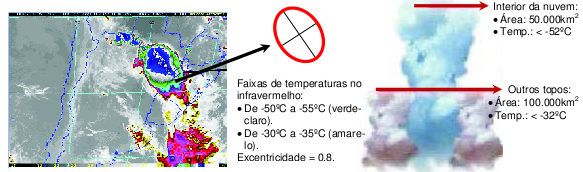
\includegraphics[height=4.5cm]{./figs/fig08.png}
\caption{À esquerda: imagem no infravermelho do satélite GOES (20030123, às 02:09 UTC). Ao centro: característica da excentricidade do CCM ocorrido nesta data. À direita: corte esquemático da nebulosidade durante um CCM.}
\FONTE{ROZANTE, 2008.}
\label{fig08}
\end{figure}

No Brasil, os CCM ocorrem mais frequentemente na região Sul, havendo também referências de se deslocarem para as regiões Sudeste e Centro-Oeste, podendo ocorrer em todas as estações do ano (SILVA DIAS, 1996). Na Figura 2.6, estão assinaladas as regiões Centro-Oeste (CO), Sudeste (SE) e Sul (SU) sob o domínio da AS. Estas são as regiões onde são observados com maior frequência a ocorrência de CCMs durante o período de estudos escolhido.

\begin{figure}
\centering
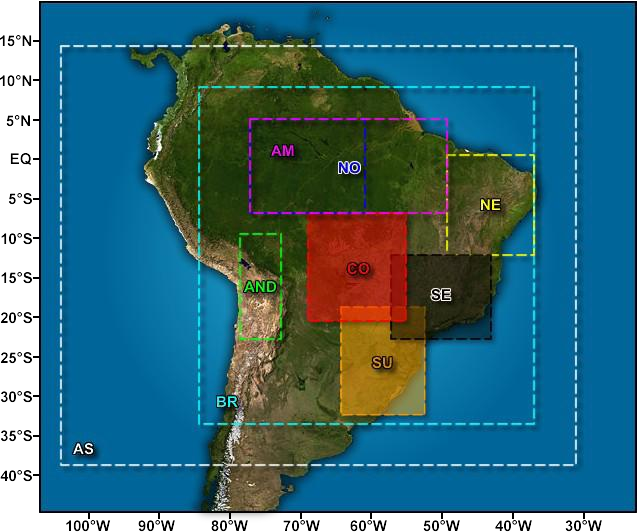
\includegraphics[height=10cm]{./figs/fig09.png}
\caption{Áreas de ocorrência de CCMs na AS.Áreas de ocorrência de CCMs na AS.}
\label{fig09}
\end{figure}

Na AS, os mecanismos de transporte de umidade da região amazônica para a região sul da AS, são a ZCAS e os Jatos de Baixos Níveis (JBN). O JBN é o principal mecanismo associado à formação e alimentação da convecção de grande parte dos CCMs (FERREIRA et al. 2003; HERDIES et al. 2002). O transporte de umidade da região amazônica em direção à região sul da AS, geralmente condensa e precipita na região de convergência do JBN, produzindo fortes correntes descendentes sob o núcleo dos CCMs, com o máximo de precipitação durante a noite (NOGUÉS-PAEGLE e BERBERY, 2000). Na Figura 2.7 é mostrado um modelo conceitual dos JBN e sua associação com a formação dos CCM (MARENGO et al., 2004).

\begin{figure}
\centering
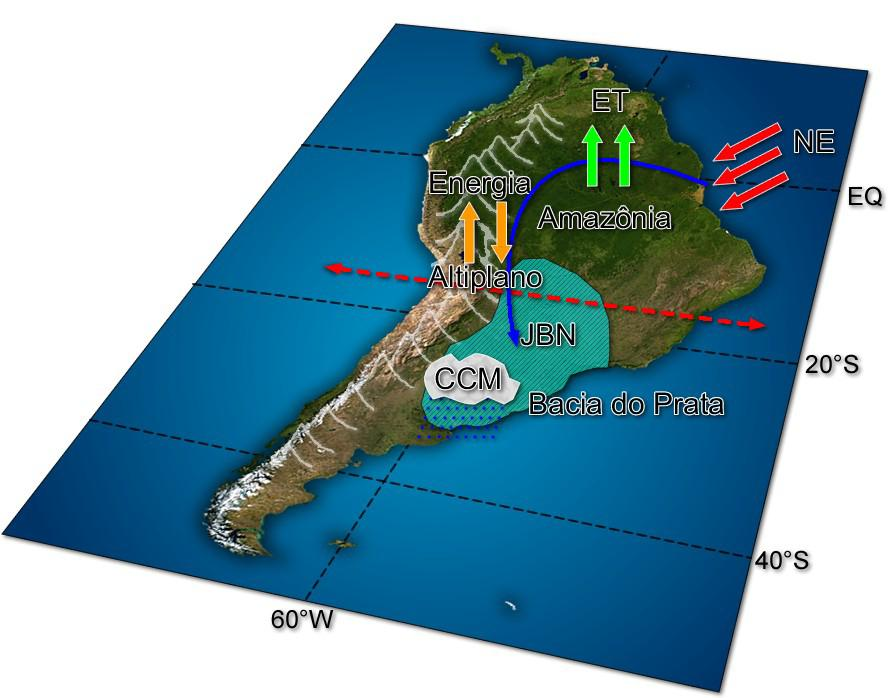
\includegraphics[height=10cm]{./figs/fig10.png}
\caption{Modelo Conceitual dos JBN. Na figura: ET - evapotranspiração; JBN - Jato de Baixos Níveis e CCM - Complexo Convectivo de Mesoescala; NE - Nordeste.}
\FONTE{adaptado de Marengo et al., 2004.}
\label{fig10}
\end{figure}
